\documentclass[twoside]{book}

% Packages required by doxygen
\usepackage{fixltx2e}
\usepackage{calc}
\usepackage{doxygen}
\usepackage[export]{adjustbox} % also loads graphicx
\usepackage{graphicx}
\usepackage[utf8]{inputenc}
\usepackage{makeidx}
\usepackage{multicol}
\usepackage{multirow}
\PassOptionsToPackage{warn}{textcomp}
\usepackage{textcomp}
\usepackage[nointegrals]{wasysym}
\usepackage[table]{xcolor}

% Font selection
\usepackage[T1]{fontenc}
\usepackage[scaled=.90]{helvet}
\usepackage{courier}
\usepackage{amssymb}
\usepackage{sectsty}
\renewcommand{\familydefault}{\sfdefault}
\allsectionsfont{%
  \fontseries{bc}\selectfont%
  \color{darkgray}%
}
\renewcommand{\DoxyLabelFont}{%
  \fontseries{bc}\selectfont%
  \color{darkgray}%
}
\newcommand{\+}{\discretionary{\mbox{\scriptsize$\hookleftarrow$}}{}{}}

% Page & text layout
\usepackage{geometry}
\geometry{%
  a4paper,%
  top=2.5cm,%
  bottom=2.5cm,%
  left=2.5cm,%
  right=2.5cm%
}
\tolerance=750
\hfuzz=15pt
\hbadness=750
\setlength{\emergencystretch}{15pt}
\setlength{\parindent}{0cm}
\setlength{\parskip}{3ex plus 2ex minus 2ex}
\makeatletter
\renewcommand{\paragraph}{%
  \@startsection{paragraph}{4}{0ex}{-1.0ex}{1.0ex}{%
    \normalfont\normalsize\bfseries\SS@parafont%
  }%
}
\renewcommand{\subparagraph}{%
  \@startsection{subparagraph}{5}{0ex}{-1.0ex}{1.0ex}{%
    \normalfont\normalsize\bfseries\SS@subparafont%
  }%
}
\makeatother

% Headers & footers
\usepackage{fancyhdr}
\pagestyle{fancyplain}
\fancyhead[LE]{\fancyplain{}{\bfseries\thepage}}
\fancyhead[CE]{\fancyplain{}{}}
\fancyhead[RE]{\fancyplain{}{\bfseries\leftmark}}
\fancyhead[LO]{\fancyplain{}{\bfseries\rightmark}}
\fancyhead[CO]{\fancyplain{}{}}
\fancyhead[RO]{\fancyplain{}{\bfseries\thepage}}
\fancyfoot[LE]{\fancyplain{}{}}
\fancyfoot[CE]{\fancyplain{}{}}
\fancyfoot[RE]{\fancyplain{}{\bfseries\scriptsize Generated by Doxygen }}
\fancyfoot[LO]{\fancyplain{}{\bfseries\scriptsize Generated by Doxygen }}
\fancyfoot[CO]{\fancyplain{}{}}
\fancyfoot[RO]{\fancyplain{}{}}
\renewcommand{\footrulewidth}{0.4pt}
\renewcommand{\chaptermark}[1]{%
  \markboth{#1}{}%
}
\renewcommand{\sectionmark}[1]{%
  \markright{\thesection\ #1}%
}

% Indices & bibliography
\usepackage{natbib}
\usepackage[titles]{tocloft}
\setcounter{tocdepth}{3}
\setcounter{secnumdepth}{5}
\makeindex

% Hyperlinks (required, but should be loaded last)
\usepackage{ifpdf}
\ifpdf
  \usepackage[pdftex,pagebackref=true]{hyperref}
\else
  \usepackage[ps2pdf,pagebackref=true]{hyperref}
\fi
\hypersetup{%
  colorlinks=true,%
  linkcolor=blue,%
  citecolor=blue,%
  unicode%
}

% Custom commands
\newcommand{\clearemptydoublepage}{%
  \newpage{\pagestyle{empty}\cleardoublepage}%
}

\usepackage{caption}
\captionsetup{labelsep=space,justification=centering,font={bf},singlelinecheck=off,skip=4pt,position=top}

%===== C O N T E N T S =====

\begin{document}

% Titlepage & ToC
\hypersetup{pageanchor=false,
             bookmarksnumbered=true,
             pdfencoding=unicode
            }
\pagenumbering{roman}
\begin{titlepage}
\vspace*{7cm}
\begin{center}%
{\Large My Project }\\
\vspace*{1cm}
{\large Generated by Doxygen 1.8.11}\\
\end{center}
\end{titlepage}
\clearemptydoublepage
\tableofcontents
\clearemptydoublepage
\pagenumbering{arabic}
\hypersetup{pageanchor=true}

%--- Begin generated contents ---
\chapter{Class Index}
\section{Class List}
Here are the classes, structs, unions and interfaces with brief descriptions\+:\begin{DoxyCompactList}
\item\contentsline{section}{\hyperlink{unionsemun}{semun} }{\pageref{unionsemun}}{}
\end{DoxyCompactList}

\chapter{File Index}
\section{File List}
Here is a list of all documented files with brief descriptions\+:\begin{DoxyCompactList}
\item\contentsline{section}{\hyperlink{Ejercicio2_8c}{Ejercicio2.\+c} \\*Ejercicio 2 de la Practica 2 }{\pageref{Ejercicio2_8c}}{}
\item\contentsline{section}{\hyperlink{Ejercicio4_8c}{Ejercicio4.\+c} \\*Ejercicio 4 de la Practica 2 }{\pageref{Ejercicio4_8c}}{}
\item\contentsline{section}{\hyperlink{Ejercicio6a_8c}{Ejercicio6a.\+c} \\*Ejercicio 6a de la Practica 2 }{\pageref{Ejercicio6a_8c}}{}
\item\contentsline{section}{\hyperlink{Ejercicio6b_8c}{Ejercicio6b.\+c} \\*Ejercicio 6b de la Practica 2 }{\pageref{Ejercicio6b_8c}}{}
\item\contentsline{section}{\hyperlink{Ejercicio8_8c}{Ejercicio8.\+c} \\*Ejercicio 8 de la Practica 2 }{\pageref{Ejercicio8_8c}}{}
\item\contentsline{section}{\hyperlink{Ejercicio8_8h}{Ejercicio8.\+h} \\*Ejercicio 8 de la Practica 2 }{\pageref{Ejercicio8_8h}}{}
\item\contentsline{section}{\hyperlink{Ejercicio9_8c}{Ejercicio9.\+c} \\*Ejercicio 9 de la Practica 2 }{\pageref{Ejercicio9_8c}}{}
\end{DoxyCompactList}

\chapter{Class Documentation}
\hypertarget{unionsemun}{}\section{semun Union Reference}
\label{unionsemun}\index{semun@{semun}}
\subsection*{Public Attributes}
\begin{DoxyCompactItemize}
\item 
int {\bfseries val}\hypertarget{unionsemun_ac6121ecb6d04a024e07e12bd71b94031}{}\label{unionsemun_ac6121ecb6d04a024e07e12bd71b94031}

\item 
struct semid\+\_\+ds $\ast$ {\bfseries semstat}\hypertarget{unionsemun_afb976847aea44952be2118ad0329d832}{}\label{unionsemun_afb976847aea44952be2118ad0329d832}

\item 
unsigned short $\ast$ {\bfseries array}\hypertarget{unionsemun_aca23b8e730a0553205813c0cb7692b54}{}\label{unionsemun_aca23b8e730a0553205813c0cb7692b54}

\end{DoxyCompactItemize}


The documentation for this union was generated from the following file\+:\begin{DoxyCompactItemize}
\item 
\hyperlink{Ejercicio8_8c}{Ejercicio8.\+c}\end{DoxyCompactItemize}

\chapter{File Documentation}
\hypertarget{Ejercicio2_8c}{}\section{Ejercicio2.\+c File Reference}
\label{Ejercicio2_8c}\index{Ejercicio2.\+c@{Ejercicio2.\+c}}


Primera parte del ejercicio 2 de la Practica 3.  


{\ttfamily \#include $<$stdio.\+h$>$}\\*
{\ttfamily \#include $<$string.\+h$>$}\\*
{\ttfamily \#include $<$sys/types.\+h$>$}\\*
{\ttfamily \#include $<$sys/wait.\+h$>$}\\*
{\ttfamily \#include $<$stdlib.\+h$>$}\\*
{\ttfamily \#include $<$unistd.\+h$>$}\\*
{\ttfamily \#include $<$signal.\+h$>$}\\*
{\ttfamily \#include $<$sys/shm.\+h$>$}\\*
{\ttfamily \#include $<$errno.\+h$>$}\\*
Include dependency graph for Ejercicio2.\+c\+:

\hypertarget{Ejercicio4_8c}{}\section{Ejercicio4.\+c File Reference}
\label{Ejercicio4_8c}\index{Ejercicio4.\+c@{Ejercicio4.\+c}}


Ejercicio 4 de la Practica 2.  


{\ttfamily \#include $<$stdio.\+h$>$}\\*
{\ttfamily \#include $<$sys/types.\+h$>$}\\*
{\ttfamily \#include $<$sys/wait.\+h$>$}\\*
{\ttfamily \#include $<$stdlib.\+h$>$}\\*
{\ttfamily \#include $<$unistd.\+h$>$}\\*
{\ttfamily \#include $<$signal.\+h$>$}\\*
Include dependency graph for Ejercicio4.\+c\+:
\nopagebreak
\begin{figure}[H]
\begin{center}
\leavevmode
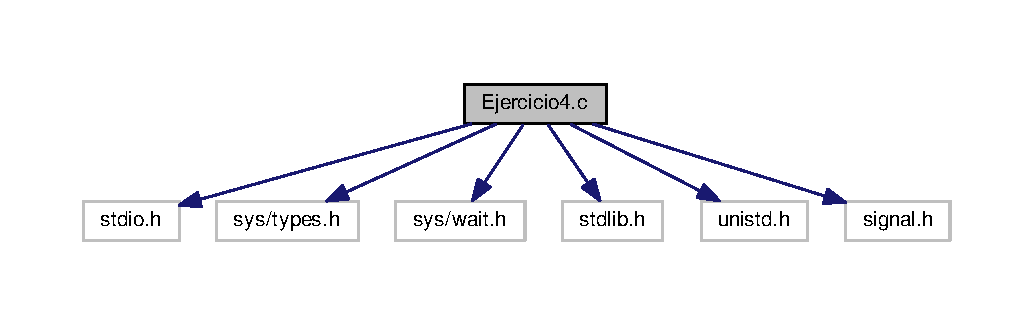
\includegraphics[width=350pt]{Ejercicio4_8c__incl}
\end{center}
\end{figure}
\subsection*{Macros}
\begin{DoxyCompactItemize}
\item 
\#define \hyperlink{Ejercicio4_8c_a9dd395f2e0046c1513c84dfcfb9e54da}{N\+U\+M\+\_\+\+H\+I\+J\+OS}~5
\end{DoxyCompactItemize}
\subsection*{Functions}
\begin{DoxyCompactItemize}
\item 
void \hyperlink{Ejercicio4_8c_a0897883a0dfdf1023f377e262cee1299}{captura} ()\hypertarget{Ejercicio4_8c_a0897883a0dfdf1023f377e262cee1299}{}\label{Ejercicio4_8c_a0897883a0dfdf1023f377e262cee1299}

\begin{DoxyCompactList}\small\item\em Funcion que ejecuta el proceso padre tras recibir la senal S\+I\+G\+U\+S\+R1. De esta forma, nos aseguramos que el proceso salga correctamente del pause() y continue su ejecucion. \end{DoxyCompactList}\item 
void \hyperlink{Ejercicio4_8c_a8dde52fc2d8703ce2fa56ebedcacee05}{terminar} ()\hypertarget{Ejercicio4_8c_a8dde52fc2d8703ce2fa56ebedcacee05}{}\label{Ejercicio4_8c_a8dde52fc2d8703ce2fa56ebedcacee05}

\begin{DoxyCompactList}\small\item\em Funcion que ejecutan los procesos hijos tras recibir la senal S\+I\+G\+U\+S\+R2, para terminar asi su ejecucion. \end{DoxyCompactList}\item 
int \hyperlink{Ejercicio4_8c_ae66f6b31b5ad750f1fe042a706a4e3d4}{main} ()
\begin{DoxyCompactList}\small\item\em El proceso padre crea un proceso hijo, que imprime 10 veces \char`\"{}\+Soy $<$\+P\+I\+D$>$ y estoy trabajando\char`\"{}, esperando un segundo entre cada vez. Una vez el proceso hijo ha impreso el texto las 10 veces, manda la señal S\+I\+G\+U\+S\+R1 al padre, que sale del pause(), y crea otro hijo, de forma que es este nuevo hijo el que manda una senal S\+I\+G\+U\+S\+R2 al hijo anterior para que este se termine a el mismo. Asi, el padre acaba creando N\+U\+M\+\_\+\+H\+I\+J\+OS procesos hijos, el mismo mata al ultimo de los hijos, y se asegura de esperar a todos. \end{DoxyCompactList}\end{DoxyCompactItemize}


\subsection{Detailed Description}
Ejercicio 4 de la Practica 2. 

\begin{DoxyAuthor}{Author}
\href{mailto:Javier.delgadod@estudiante.uam.es}{\tt Javier.\+delgadod@estudiante.\+uam.\+es} 

\href{mailto:Javier.lopezcano@estudiante.uam.es}{\tt Javier.\+lopezcano@estudiante.\+uam.\+es} 
\end{DoxyAuthor}


\subsection{Macro Definition Documentation}
\index{Ejercicio4.\+c@{Ejercicio4.\+c}!N\+U\+M\+\_\+\+H\+I\+J\+OS@{N\+U\+M\+\_\+\+H\+I\+J\+OS}}
\index{N\+U\+M\+\_\+\+H\+I\+J\+OS@{N\+U\+M\+\_\+\+H\+I\+J\+OS}!Ejercicio4.\+c@{Ejercicio4.\+c}}
\subsubsection[{\texorpdfstring{N\+U\+M\+\_\+\+H\+I\+J\+OS}{NUM_HIJOS}}]{\setlength{\rightskip}{0pt plus 5cm}\#define N\+U\+M\+\_\+\+H\+I\+J\+OS~5}\hypertarget{Ejercicio4_8c_a9dd395f2e0046c1513c84dfcfb9e54da}{}\label{Ejercicio4_8c_a9dd395f2e0046c1513c84dfcfb9e54da}
Numero de hijos que crea el proceso padre 

\subsection{Function Documentation}
\index{Ejercicio4.\+c@{Ejercicio4.\+c}!main@{main}}
\index{main@{main}!Ejercicio4.\+c@{Ejercicio4.\+c}}
\subsubsection[{\texorpdfstring{main()}{main()}}]{\setlength{\rightskip}{0pt plus 5cm}int main (
\begin{DoxyParamCaption}
\item[{void}]{}
\end{DoxyParamCaption}
)}\hypertarget{Ejercicio4_8c_ae66f6b31b5ad750f1fe042a706a4e3d4}{}\label{Ejercicio4_8c_ae66f6b31b5ad750f1fe042a706a4e3d4}


El proceso padre crea un proceso hijo, que imprime 10 veces \char`\"{}\+Soy $<$\+P\+I\+D$>$ y estoy trabajando\char`\"{}, esperando un segundo entre cada vez. Una vez el proceso hijo ha impreso el texto las 10 veces, manda la señal S\+I\+G\+U\+S\+R1 al padre, que sale del pause(), y crea otro hijo, de forma que es este nuevo hijo el que manda una senal S\+I\+G\+U\+S\+R2 al hijo anterior para que este se termine a el mismo. Asi, el padre acaba creando N\+U\+M\+\_\+\+H\+I\+J\+OS procesos hijos, el mismo mata al ultimo de los hijos, y se asegura de esperar a todos. 

\begin{DoxyReturn}{Returns}
int que determina si el programa se ha ejecutado o no con exito. 
\end{DoxyReturn}

\hypertarget{Ejercicio6a_8c}{}\section{Ejercicio6a.\+c File Reference}
\label{Ejercicio6a_8c}\index{Ejercicio6a.\+c@{Ejercicio6a.\+c}}


Ejercicio 6a de la Practica 2.  


{\ttfamily \#include $<$stdio.\+h$>$}\\*
{\ttfamily \#include $<$sys/types.\+h$>$}\\*
{\ttfamily \#include $<$sys/wait.\+h$>$}\\*
{\ttfamily \#include $<$stdlib.\+h$>$}\\*
{\ttfamily \#include $<$unistd.\+h$>$}\\*
{\ttfamily \#include $<$signal.\+h$>$}\\*
{\ttfamily \#include $<$time.\+h$>$}\\*
Include dependency graph for Ejercicio6a.\+c\+:
\nopagebreak
\begin{figure}[H]
\begin{center}
\leavevmode
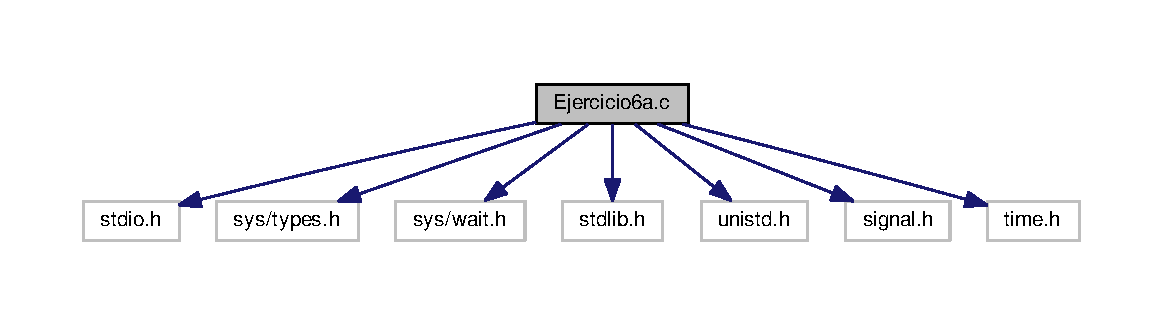
\includegraphics[width=350pt]{Ejercicio6a_8c__incl}
\end{center}
\end{figure}
\subsection*{Macros}
\begin{DoxyCompactItemize}
\item 
\#define {\bfseries N\+U\+M\+\_\+\+P\+R\+OC}~5\hypertarget{Ejercicio6a_8c_acee2369f62e4a096d243dec3cd7d0b00}{}\label{Ejercicio6a_8c_acee2369f62e4a096d243dec3cd7d0b00}

\end{DoxyCompactItemize}
\subsection*{Functions}
\begin{DoxyCompactItemize}
\item 
int \hyperlink{Ejercicio6a_8c_a840291bc02cba5474a4cb46a9b9566fe}{main} (void)
\begin{DoxyCompactList}\small\item\em El proceso padre crea un proceso hijo, que inicializa una mascara vacia e introduce en ella las senales S\+I\+G\+U\+S\+R1, S\+I\+G\+U\+S\+R2, S\+I\+G\+U\+S\+R3 y lanza un alarm que mandara una señal a los 40 segundos Tras esto entra en un while(1) y bloquea las señales para que si le llegan durante la cuenta que realizara a continuacion, no se pare esta y comienza a imprimir 0 1 2 3 4 y a esperar 1 segundo y 3 segundos continuamente, pero antes de esperar los 3 segundos, desbloquea las senales de modo que si ha recibido la senal del alarm, se para su ejecucion tras lo cual acaba tambien el proceso padre que habia hecho un wait para esperar al hijo. \end{DoxyCompactList}\end{DoxyCompactItemize}


\subsection{Detailed Description}
Ejercicio 6a de la Practica 2. 

\begin{DoxyAuthor}{Author}
\href{mailto:Javier.delgadod@estudiante.uam.es}{\tt Javier.\+delgadod@estudiante.\+uam.\+es} 

\href{mailto:Javier.lopezcano@estudiante.uam.es}{\tt Javier.\+lopezcano@estudiante.\+uam.\+es} 
\end{DoxyAuthor}


\subsection{Function Documentation}
\index{Ejercicio6a.\+c@{Ejercicio6a.\+c}!main@{main}}
\index{main@{main}!Ejercicio6a.\+c@{Ejercicio6a.\+c}}
\subsubsection[{\texorpdfstring{main(void)}{main(void)}}]{\setlength{\rightskip}{0pt plus 5cm}int main (
\begin{DoxyParamCaption}
\item[{void}]{}
\end{DoxyParamCaption}
)}\hypertarget{Ejercicio6a_8c_a840291bc02cba5474a4cb46a9b9566fe}{}\label{Ejercicio6a_8c_a840291bc02cba5474a4cb46a9b9566fe}


El proceso padre crea un proceso hijo, que inicializa una mascara vacia e introduce en ella las senales S\+I\+G\+U\+S\+R1, S\+I\+G\+U\+S\+R2, S\+I\+G\+U\+S\+R3 y lanza un alarm que mandara una señal a los 40 segundos Tras esto entra en un while(1) y bloquea las señales para que si le llegan durante la cuenta que realizara a continuacion, no se pare esta y comienza a imprimir 0 1 2 3 4 y a esperar 1 segundo y 3 segundos continuamente, pero antes de esperar los 3 segundos, desbloquea las senales de modo que si ha recibido la senal del alarm, se para su ejecucion tras lo cual acaba tambien el proceso padre que habia hecho un wait para esperar al hijo. 

\begin{DoxyReturn}{Returns}
int que determina si el programa se ha ejecutado o no con exito. 
\end{DoxyReturn}

\hypertarget{Ejercicio6b_8c}{}\section{Ejercicio6b.\+c File Reference}
\label{Ejercicio6b_8c}\index{Ejercicio6b.\+c@{Ejercicio6b.\+c}}


Ejercicio 6b de la Practica 2.  


{\ttfamily \#include $<$stdio.\+h$>$}\\*
{\ttfamily \#include $<$sys/types.\+h$>$}\\*
{\ttfamily \#include $<$sys/wait.\+h$>$}\\*
{\ttfamily \#include $<$stdlib.\+h$>$}\\*
{\ttfamily \#include $<$unistd.\+h$>$}\\*
{\ttfamily \#include $<$signal.\+h$>$}\\*
{\ttfamily \#include $<$time.\+h$>$}\\*
Include dependency graph for Ejercicio6b.\+c\+:
\nopagebreak
\begin{figure}[H]
\begin{center}
\leavevmode
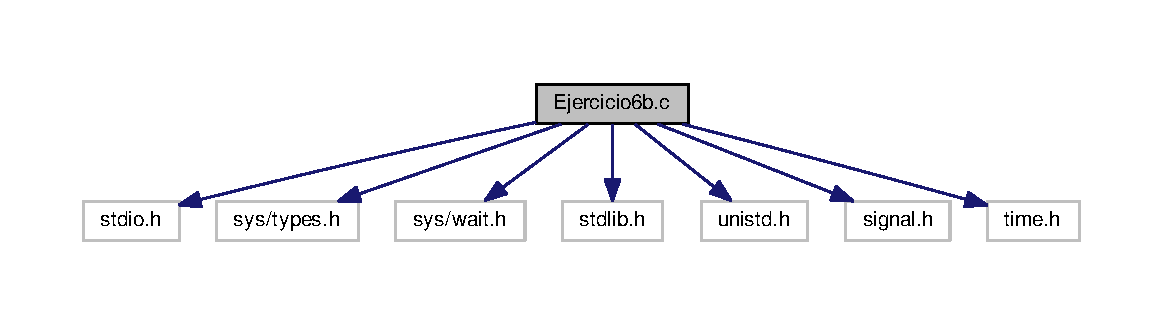
\includegraphics[width=350pt]{Ejercicio6b_8c__incl}
\end{center}
\end{figure}
\subsection*{Macros}
\begin{DoxyCompactItemize}
\item 
\#define {\bfseries N\+U\+M\+\_\+\+P\+R\+OC}~5\hypertarget{Ejercicio6b_8c_acee2369f62e4a096d243dec3cd7d0b00}{}\label{Ejercicio6b_8c_acee2369f62e4a096d243dec3cd7d0b00}

\end{DoxyCompactItemize}
\subsection*{Functions}
\begin{DoxyCompactItemize}
\item 
void \hyperlink{Ejercicio6b_8c_a3d60508a7c724aae98e027b714db086a}{recibir\+S\+I\+G\+T\+E\+RM} ()\hypertarget{Ejercicio6b_8c_a3d60508a7c724aae98e027b714db086a}{}\label{Ejercicio6b_8c_a3d60508a7c724aae98e027b714db086a}

\begin{DoxyCompactList}\small\item\em Esta funcion determina el funcionamiento que tendra el hijo tras recibir la senal S\+I\+G\+T\+E\+RM. En este caso al recibir esta senal el proceso hijo ejecutara esta funcion que hara que imprima Soy $<$\+P\+I\+D$>$ y he recibido la señal S\+I\+G\+T\+E\+RM y termine su ejecucion. \end{DoxyCompactList}\item 
int \hyperlink{Ejercicio6b_8c_a840291bc02cba5474a4cb46a9b9566fe}{main} (void)
\begin{DoxyCompactList}\small\item\em El proceso padre crea un proceso hijo, que inicializa una funcion que maneja la senal S\+I\+G\+T\+E\+RM (define lo que tiene que hacer el proceso hijo al recibir esta senal), y comienza a realizar lo mismo que en el ejercicio 6a, imprimir 0 1 2 3 4 y esperar 1 segundo y 3 segundos continuamente. El proceso padre tras lanzar el hijo duerme 40 segundos, y al pasar este tiempo lanza la senal S\+I\+G\+T\+E\+RM al hijo y realiza un wait para esperar a que el hijo acabe, tras lo cual acaba su ejecucion. \end{DoxyCompactList}\end{DoxyCompactItemize}


\subsection{Detailed Description}
Ejercicio 6b de la Practica 2. 

\begin{DoxyAuthor}{Author}
\href{mailto:Javier.delgadod@estudiante.uam.es}{\tt Javier.\+delgadod@estudiante.\+uam.\+es} 

\href{mailto:Javier.lopezcano@estudiante.uam.es}{\tt Javier.\+lopezcano@estudiante.\+uam.\+es} 
\end{DoxyAuthor}


\subsection{Function Documentation}
\index{Ejercicio6b.\+c@{Ejercicio6b.\+c}!main@{main}}
\index{main@{main}!Ejercicio6b.\+c@{Ejercicio6b.\+c}}
\subsubsection[{\texorpdfstring{main(void)}{main(void)}}]{\setlength{\rightskip}{0pt plus 5cm}int main (
\begin{DoxyParamCaption}
\item[{void}]{}
\end{DoxyParamCaption}
)}\hypertarget{Ejercicio6b_8c_a840291bc02cba5474a4cb46a9b9566fe}{}\label{Ejercicio6b_8c_a840291bc02cba5474a4cb46a9b9566fe}


El proceso padre crea un proceso hijo, que inicializa una funcion que maneja la senal S\+I\+G\+T\+E\+RM (define lo que tiene que hacer el proceso hijo al recibir esta senal), y comienza a realizar lo mismo que en el ejercicio 6a, imprimir 0 1 2 3 4 y esperar 1 segundo y 3 segundos continuamente. El proceso padre tras lanzar el hijo duerme 40 segundos, y al pasar este tiempo lanza la senal S\+I\+G\+T\+E\+RM al hijo y realiza un wait para esperar a que el hijo acabe, tras lo cual acaba su ejecucion. 

\begin{DoxyReturn}{Returns}
int que determina si el programa se ha ejecutado o no con exito. 
\end{DoxyReturn}

\hypertarget{Ejercicio8_8c}{}\section{Ejercicio8.\+c File Reference}
\label{Ejercicio8_8c}\index{Ejercicio8.\+c@{Ejercicio8.\+c}}


Ejercicio 8 de la Practica 2.  


{\ttfamily \#include $<$stdio.\+h$>$}\\*
{\ttfamily \#include $<$sys/types.\+h$>$}\\*
{\ttfamily \#include $<$sys/ipc.\+h$>$}\\*
{\ttfamily \#include $<$sys/sem.\+h$>$}\\*
{\ttfamily \#include $<$errno.\+h$>$}\\*
{\ttfamily \#include $<$sys/shm.\+h$>$}\\*
{\ttfamily \#include $<$stdlib.\+h$>$}\\*
{\ttfamily \#include \char`\"{}Ejercicio8.\+h\char`\"{}}\\*
Include dependency graph for Ejercicio8.\+c\+:
\nopagebreak
\begin{figure}[H]
\begin{center}
\leavevmode
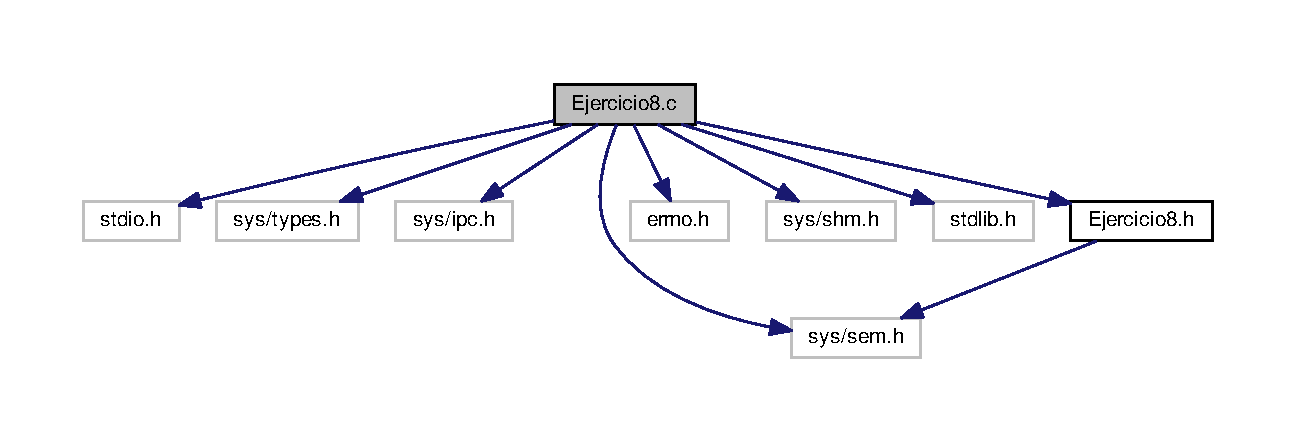
\includegraphics[width=350pt]{Ejercicio8_8c__incl}
\end{center}
\end{figure}
\subsection*{Classes}
\begin{DoxyCompactItemize}
\item 
union \hyperlink{unionsemun}{semun}
\end{DoxyCompactItemize}
\subsection*{Macros}
\begin{DoxyCompactItemize}
\item 
\#define {\bfseries S\+E\+M\+K\+EY}~75798\hypertarget{Ejercicio8_8c_ada831b9e37399bf906c8184a888e28cd}{}\label{Ejercicio8_8c_ada831b9e37399bf906c8184a888e28cd}

\item 
\#define {\bfseries N\+\_\+\+S\+E\+M\+A\+F\+O\+R\+OS}~2\hypertarget{Ejercicio8_8c_a95c81905ff3d55e62fb763f407f9fab1}{}\label{Ejercicio8_8c_a95c81905ff3d55e62fb763f407f9fab1}

\end{DoxyCompactItemize}
\subsection*{Functions}
\begin{DoxyCompactItemize}
\item 
int \hyperlink{Ejercicio8_8c_a4af104b0ed37e6ae0289a1059bc6e990}{Inicializar\+\_\+\+Semaforo} (int semid, unsigned short $\ast$array)
\begin{DoxyCompactList}\small\item\em Función que inicializa un array de semaforos con id semid y con los valores que se pasan a traves del array de shorts. \end{DoxyCompactList}\item 
int \hyperlink{Ejercicio8_8c_a731339337960a681efa435a10f12c312}{Borrar\+\_\+\+Semaforo} (int semid)
\begin{DoxyCompactList}\small\item\em Función que elimina un array de semaforos. \end{DoxyCompactList}\item 
int \hyperlink{Ejercicio8_8c_a16b16dd895b5f4cbe48f1ac8977e8b35}{Crear\+\_\+\+Semaforo} (key\+\_\+t key, int size, int $\ast$semid)
\begin{DoxyCompactList}\small\item\em Funcion que crea un array de semaforos. \end{DoxyCompactList}\item 
int \hyperlink{Ejercicio8_8c_a883244cd3b83c42cda23687da1b63369}{Down\+\_\+\+Semaforo} (int id, int num\+\_\+sem, int undo)
\begin{DoxyCompactList}\small\item\em Funcion que baja un semaforo. \end{DoxyCompactList}\item 
int \hyperlink{Ejercicio8_8c_ab375ebfc38acbdced46e062a689d5fad}{Down\+Multiple\+\_\+\+Semaforo} (int id, int size, int undo, int $\ast$active)
\begin{DoxyCompactList}\small\item\em Funcion que baja varios semaforos de un array llamando varias veces a Down\+\_\+\+Semaforo. \end{DoxyCompactList}\item 
int \hyperlink{Ejercicio8_8c_a2d5e735aecee4f493898b3d4ebab1a10}{Up\+\_\+\+Semaforo} (int id, int num\+\_\+sem, int undo)
\begin{DoxyCompactList}\small\item\em Funcion que sube un semaforo. \end{DoxyCompactList}\item 
int \hyperlink{Ejercicio8_8c_a943759695f018d64a94b8a2c49308092}{Up\+Multiple\+\_\+\+Semaforo} (int id, int size, int undo, int $\ast$active)
\begin{DoxyCompactList}\small\item\em Funcion que sube varios semaforos de un array llamando varias veces a Up\+\_\+\+Semaforo. \end{DoxyCompactList}\item 
int \hyperlink{Ejercicio8_8c_ac8da963855e09bf929c085486f4a3b47}{test} ()
\begin{DoxyCompactList}\small\item\em Programa que prueba el funcionamiento de la libreria. \end{DoxyCompactList}\end{DoxyCompactItemize}
\subsection*{Variables}
\begin{DoxyCompactItemize}
\item 
union \hyperlink{unionsemun}{semun} {\bfseries arg}\hypertarget{Ejercicio8_8c_a7c4d098a46a7276dc49238b0590c594a}{}\label{Ejercicio8_8c_a7c4d098a46a7276dc49238b0590c594a}

\end{DoxyCompactItemize}


\subsection{Detailed Description}
Ejercicio 8 de la Practica 2. 

\begin{DoxyAuthor}{Author}
\href{mailto:Javier.delgadod@estudiante.uam.es}{\tt Javier.\+delgadod@estudiante.\+uam.\+es} 

\href{mailto:Javier.lopezcano@estudiante.uam.es}{\tt Javier.\+lopezcano@estudiante.\+uam.\+es} 
\end{DoxyAuthor}


\subsection{Function Documentation}
\index{Ejercicio8.\+c@{Ejercicio8.\+c}!Borrar\+\_\+\+Semaforo@{Borrar\+\_\+\+Semaforo}}
\index{Borrar\+\_\+\+Semaforo@{Borrar\+\_\+\+Semaforo}!Ejercicio8.\+c@{Ejercicio8.\+c}}
\subsubsection[{\texorpdfstring{Borrar\+\_\+\+Semaforo(int semid)}{Borrar_Semaforo(int semid)}}]{\setlength{\rightskip}{0pt plus 5cm}int Borrar\+\_\+\+Semaforo (
\begin{DoxyParamCaption}
\item[{int}]{semid}
\end{DoxyParamCaption}
)}\hypertarget{Ejercicio8_8c_a731339337960a681efa435a10f12c312}{}\label{Ejercicio8_8c_a731339337960a681efa435a10f12c312}


Función que elimina un array de semaforos. 


\begin{DoxyParams}{Parameters}
{\em semid} & Int que es el id del array de semáforos. \\
\hline
\end{DoxyParams}
\begin{DoxyReturn}{Returns}
int que determina si la funcion se ha ejecutado o no con exito. 
\end{DoxyReturn}
\index{Ejercicio8.\+c@{Ejercicio8.\+c}!Crear\+\_\+\+Semaforo@{Crear\+\_\+\+Semaforo}}
\index{Crear\+\_\+\+Semaforo@{Crear\+\_\+\+Semaforo}!Ejercicio8.\+c@{Ejercicio8.\+c}}
\subsubsection[{\texorpdfstring{Crear\+\_\+\+Semaforo(key\+\_\+t key, int size, int $\ast$semid)}{Crear_Semaforo(key_t key, int size, int *semid)}}]{\setlength{\rightskip}{0pt plus 5cm}int Crear\+\_\+\+Semaforo (
\begin{DoxyParamCaption}
\item[{key\+\_\+t}]{key, }
\item[{int}]{size, }
\item[{int $\ast$}]{semid}
\end{DoxyParamCaption}
)}\hypertarget{Ejercicio8_8c_a16b16dd895b5f4cbe48f1ac8977e8b35}{}\label{Ejercicio8_8c_a16b16dd895b5f4cbe48f1ac8977e8b35}


Funcion que crea un array de semaforos. 


\begin{DoxyParams}{Parameters}
{\em key} & Identificador de I\+PC. \\
\hline
{\em size} & Tamano del array de semaforos que se quiere crear. \\
\hline
{\em semid} & Int que es el id del array de semáforos. \\
\hline
\end{DoxyParams}
\begin{DoxyReturn}{Returns}
int que determina si la funcion se ha ejecutado o no con exito. 
\end{DoxyReturn}
\index{Ejercicio8.\+c@{Ejercicio8.\+c}!Down\+\_\+\+Semaforo@{Down\+\_\+\+Semaforo}}
\index{Down\+\_\+\+Semaforo@{Down\+\_\+\+Semaforo}!Ejercicio8.\+c@{Ejercicio8.\+c}}
\subsubsection[{\texorpdfstring{Down\+\_\+\+Semaforo(int id, int num\+\_\+sem, int undo)}{Down_Semaforo(int id, int num_sem, int undo)}}]{\setlength{\rightskip}{0pt plus 5cm}int Down\+\_\+\+Semaforo (
\begin{DoxyParamCaption}
\item[{int}]{id, }
\item[{int}]{num\+\_\+sem, }
\item[{int}]{undo}
\end{DoxyParamCaption}
)}\hypertarget{Ejercicio8_8c_a883244cd3b83c42cda23687da1b63369}{}\label{Ejercicio8_8c_a883244cd3b83c42cda23687da1b63369}


Funcion que baja un semaforo. 


\begin{DoxyParams}{Parameters}
{\em id} & Int con el id del array de semaforos. \\
\hline
{\em num\+\_\+sem} & Int con el indice del semaforo que se quiere bajar. \\
\hline
{\em undo} & Int que es la bandera que hay que usar en la estructura sem\+\_\+oper. \\
\hline
\end{DoxyParams}
\begin{DoxyReturn}{Returns}
int que determina si la funcion se ha ejecutado o no con exito. 
\end{DoxyReturn}
\index{Ejercicio8.\+c@{Ejercicio8.\+c}!Down\+Multiple\+\_\+\+Semaforo@{Down\+Multiple\+\_\+\+Semaforo}}
\index{Down\+Multiple\+\_\+\+Semaforo@{Down\+Multiple\+\_\+\+Semaforo}!Ejercicio8.\+c@{Ejercicio8.\+c}}
\subsubsection[{\texorpdfstring{Down\+Multiple\+\_\+\+Semaforo(int id, int size, int undo, int $\ast$active)}{DownMultiple_Semaforo(int id, int size, int undo, int *active)}}]{\setlength{\rightskip}{0pt plus 5cm}int Down\+Multiple\+\_\+\+Semaforo (
\begin{DoxyParamCaption}
\item[{int}]{id, }
\item[{int}]{size, }
\item[{int}]{undo, }
\item[{int $\ast$}]{active}
\end{DoxyParamCaption}
)}\hypertarget{Ejercicio8_8c_ab375ebfc38acbdced46e062a689d5fad}{}\label{Ejercicio8_8c_ab375ebfc38acbdced46e062a689d5fad}


Funcion que baja varios semaforos de un array llamando varias veces a Down\+\_\+\+Semaforo. 


\begin{DoxyParams}{Parameters}
{\em id} & Int con el id del array de semaforos. \\
\hline
{\em size} & Int con el tamano del array de semaforos. \\
\hline
{\em undo} & Int que es la bandera que hay que usar en la estructura sem\+\_\+oper. \\
\hline
{\em active} & Array de int con los indices de los semaforos que se quiere bajar. \\
\hline
\end{DoxyParams}
\begin{DoxyReturn}{Returns}
int que determina si la funcion se ha ejecutado o no con exito. 
\end{DoxyReturn}
\index{Ejercicio8.\+c@{Ejercicio8.\+c}!Inicializar\+\_\+\+Semaforo@{Inicializar\+\_\+\+Semaforo}}
\index{Inicializar\+\_\+\+Semaforo@{Inicializar\+\_\+\+Semaforo}!Ejercicio8.\+c@{Ejercicio8.\+c}}
\subsubsection[{\texorpdfstring{Inicializar\+\_\+\+Semaforo(int semid, unsigned short $\ast$array)}{Inicializar_Semaforo(int semid, unsigned short *array)}}]{\setlength{\rightskip}{0pt plus 5cm}int Inicializar\+\_\+\+Semaforo (
\begin{DoxyParamCaption}
\item[{int}]{semid, }
\item[{unsigned short $\ast$}]{array}
\end{DoxyParamCaption}
)}\hypertarget{Ejercicio8_8c_a4af104b0ed37e6ae0289a1059bc6e990}{}\label{Ejercicio8_8c_a4af104b0ed37e6ae0289a1059bc6e990}


Función que inicializa un array de semaforos con id semid y con los valores que se pasan a traves del array de shorts. 


\begin{DoxyParams}{Parameters}
{\em semid} & Int que es el id del array de semaforos. \\
\hline
{\em array} & Array de shorts con la informacion para inicializar los semaforos. \\
\hline
\end{DoxyParams}
\begin{DoxyReturn}{Returns}
int que determina si la funcion se ha ejecutado o no con exito. 
\end{DoxyReturn}
\index{Ejercicio8.\+c@{Ejercicio8.\+c}!test@{test}}
\index{test@{test}!Ejercicio8.\+c@{Ejercicio8.\+c}}
\subsubsection[{\texorpdfstring{test()}{test()}}]{\setlength{\rightskip}{0pt plus 5cm}int test (
\begin{DoxyParamCaption}
{}
\end{DoxyParamCaption}
)}\hypertarget{Ejercicio8_8c_ac8da963855e09bf929c085486f4a3b47}{}\label{Ejercicio8_8c_ac8da963855e09bf929c085486f4a3b47}


Programa que prueba el funcionamiento de la libreria. 

\begin{DoxyReturn}{Returns}
int que determina si el programa se ha ejecutado o no con exito. 
\end{DoxyReturn}
\index{Ejercicio8.\+c@{Ejercicio8.\+c}!Up\+\_\+\+Semaforo@{Up\+\_\+\+Semaforo}}
\index{Up\+\_\+\+Semaforo@{Up\+\_\+\+Semaforo}!Ejercicio8.\+c@{Ejercicio8.\+c}}
\subsubsection[{\texorpdfstring{Up\+\_\+\+Semaforo(int id, int num\+\_\+sem, int undo)}{Up_Semaforo(int id, int num_sem, int undo)}}]{\setlength{\rightskip}{0pt plus 5cm}int Up\+\_\+\+Semaforo (
\begin{DoxyParamCaption}
\item[{int}]{id, }
\item[{int}]{num\+\_\+sem, }
\item[{int}]{undo}
\end{DoxyParamCaption}
)}\hypertarget{Ejercicio8_8c_a2d5e735aecee4f493898b3d4ebab1a10}{}\label{Ejercicio8_8c_a2d5e735aecee4f493898b3d4ebab1a10}


Funcion que sube un semaforo. 


\begin{DoxyParams}{Parameters}
{\em id} & Int con el id del array de semaforos. \\
\hline
{\em num\+\_\+sem} & Int con el indice del semaforo que se quiere subir. \\
\hline
{\em undo} & Int que es la bandera que hay que usar en la estructura sem\+\_\+oper. \\
\hline
\end{DoxyParams}
\begin{DoxyReturn}{Returns}
int que determina si la funcion se ha ejecutado o no con exito. 
\end{DoxyReturn}
\index{Ejercicio8.\+c@{Ejercicio8.\+c}!Up\+Multiple\+\_\+\+Semaforo@{Up\+Multiple\+\_\+\+Semaforo}}
\index{Up\+Multiple\+\_\+\+Semaforo@{Up\+Multiple\+\_\+\+Semaforo}!Ejercicio8.\+c@{Ejercicio8.\+c}}
\subsubsection[{\texorpdfstring{Up\+Multiple\+\_\+\+Semaforo(int id, int size, int undo, int $\ast$active)}{UpMultiple_Semaforo(int id, int size, int undo, int *active)}}]{\setlength{\rightskip}{0pt plus 5cm}int Up\+Multiple\+\_\+\+Semaforo (
\begin{DoxyParamCaption}
\item[{int}]{id, }
\item[{int}]{size, }
\item[{int}]{undo, }
\item[{int $\ast$}]{active}
\end{DoxyParamCaption}
)}\hypertarget{Ejercicio8_8c_a943759695f018d64a94b8a2c49308092}{}\label{Ejercicio8_8c_a943759695f018d64a94b8a2c49308092}


Funcion que sube varios semaforos de un array llamando varias veces a Up\+\_\+\+Semaforo. 


\begin{DoxyParams}{Parameters}
{\em id} & Int con el id del array de semaforos. \\
\hline
{\em size} & Int con el tamano del array de semaforos. \\
\hline
{\em undo} & Int que es la bandera que hay que usar en la estructura sem\+\_\+oper. \\
\hline
{\em active} & Array de int con los indices de los semaforos que se quiere subir. \\
\hline
\end{DoxyParams}
\begin{DoxyReturn}{Returns}
int que determina si la funcion se ha ejecutado o no con exito. 
\end{DoxyReturn}

\hypertarget{Ejercicio8_8h}{}\section{Ejercicio8.\+h File Reference}
\label{Ejercicio8_8h}\index{Ejercicio8.\+h@{Ejercicio8.\+h}}


Ejercicio 8 de la Practica 2.  


{\ttfamily \#include $<$sys/sem.\+h$>$}\\*
Include dependency graph for Ejercicio8.\+h\+:
\nopagebreak
\begin{figure}[H]
\begin{center}
\leavevmode
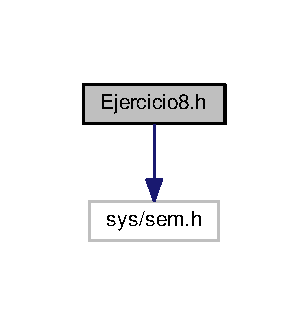
\includegraphics[width=148pt]{Ejercicio8_8h__incl}
\end{center}
\end{figure}
This graph shows which files directly or indirectly include this file\+:
\nopagebreak
\begin{figure}[H]
\begin{center}
\leavevmode
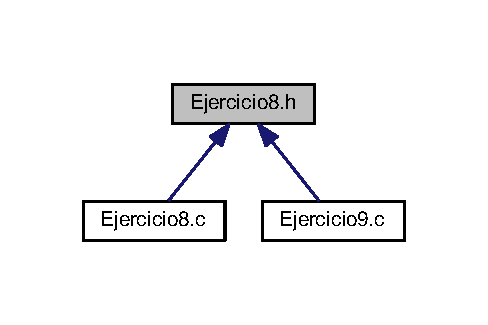
\includegraphics[width=234pt]{Ejercicio8_8h__dep__incl}
\end{center}
\end{figure}
\subsection*{Macros}
\begin{DoxyCompactItemize}
\item 
\#define {\bfseries E\+R\+R\+OR}~-\/1\hypertarget{Ejercicio8_8h_a8fe83ac76edc595f6b98cd4a4127aed5}{}\label{Ejercicio8_8h_a8fe83ac76edc595f6b98cd4a4127aed5}

\item 
\#define {\bfseries OK}~0\hypertarget{Ejercicio8_8h_aba51915c87d64af47fb1cc59348961c9}{}\label{Ejercicio8_8h_aba51915c87d64af47fb1cc59348961c9}

\item 
\#define {\bfseries C\+R\+E\+A\+DO}~1\hypertarget{Ejercicio8_8h_a00182e3826731997fd4a69a493fac3dd}{}\label{Ejercicio8_8h_a00182e3826731997fd4a69a493fac3dd}

\end{DoxyCompactItemize}
\subsection*{Functions}
\begin{DoxyCompactItemize}
\item 
int \hyperlink{Ejercicio8_8h_a4af104b0ed37e6ae0289a1059bc6e990}{Inicializar\+\_\+\+Semaforo} (int semid, unsigned short $\ast$array)
\begin{DoxyCompactList}\small\item\em Función que inicializa un array de semaforos con id semid y con los valores que se pasan a traves del array de shorts. \end{DoxyCompactList}\item 
int \hyperlink{Ejercicio8_8h_a731339337960a681efa435a10f12c312}{Borrar\+\_\+\+Semaforo} (int semid)
\begin{DoxyCompactList}\small\item\em Función que elimina un array de semaforos. \end{DoxyCompactList}\item 
int \hyperlink{Ejercicio8_8h_a16b16dd895b5f4cbe48f1ac8977e8b35}{Crear\+\_\+\+Semaforo} (key\+\_\+t key, int size, int $\ast$semid)
\begin{DoxyCompactList}\small\item\em Funcion que crea un array de semaforos. \end{DoxyCompactList}\item 
int \hyperlink{Ejercicio8_8h_a883244cd3b83c42cda23687da1b63369}{Down\+\_\+\+Semaforo} (int id, int num\+\_\+sem, int undo)
\begin{DoxyCompactList}\small\item\em Funcion que baja un semaforo. \end{DoxyCompactList}\item 
int \hyperlink{Ejercicio8_8h_ab375ebfc38acbdced46e062a689d5fad}{Down\+Multiple\+\_\+\+Semaforo} (int id, int size, int undo, int $\ast$active)
\begin{DoxyCompactList}\small\item\em Funcion que baja varios semaforos de un array llamando varias veces a Down\+\_\+\+Semaforo. \end{DoxyCompactList}\item 
int \hyperlink{Ejercicio8_8h_a2d5e735aecee4f493898b3d4ebab1a10}{Up\+\_\+\+Semaforo} (int id, int num\+\_\+sem, int undo)
\begin{DoxyCompactList}\small\item\em Funcion que sube un semaforo. \end{DoxyCompactList}\item 
int \hyperlink{Ejercicio8_8h_a943759695f018d64a94b8a2c49308092}{Up\+Multiple\+\_\+\+Semaforo} (int id, int size, int undo, int $\ast$active)
\begin{DoxyCompactList}\small\item\em Funcion que sube varios semaforos de un array llamando varias veces a Up\+\_\+\+Semaforo. \end{DoxyCompactList}\end{DoxyCompactItemize}


\subsection{Detailed Description}
Ejercicio 8 de la Practica 2. 

\begin{DoxyAuthor}{Author}
\href{mailto:Javier.delgadod@estudiante.uam.es}{\tt Javier.\+delgadod@estudiante.\+uam.\+es} 

\href{mailto:Javier.lopezcano@estudiante.uam.es}{\tt Javier.\+lopezcano@estudiante.\+uam.\+es} 
\end{DoxyAuthor}


\subsection{Function Documentation}
\index{Ejercicio8.\+h@{Ejercicio8.\+h}!Borrar\+\_\+\+Semaforo@{Borrar\+\_\+\+Semaforo}}
\index{Borrar\+\_\+\+Semaforo@{Borrar\+\_\+\+Semaforo}!Ejercicio8.\+h@{Ejercicio8.\+h}}
\subsubsection[{\texorpdfstring{Borrar\+\_\+\+Semaforo(int semid)}{Borrar_Semaforo(int semid)}}]{\setlength{\rightskip}{0pt plus 5cm}int Borrar\+\_\+\+Semaforo (
\begin{DoxyParamCaption}
\item[{int}]{semid}
\end{DoxyParamCaption}
)}\hypertarget{Ejercicio8_8h_a731339337960a681efa435a10f12c312}{}\label{Ejercicio8_8h_a731339337960a681efa435a10f12c312}


Función que elimina un array de semaforos. 


\begin{DoxyParams}{Parameters}
{\em semid} & Int que es el id del array de semáforos. \\
\hline
\end{DoxyParams}
\begin{DoxyReturn}{Returns}
int que determina si la funcion se ha ejecutado o no con exito. 
\end{DoxyReturn}
\index{Ejercicio8.\+h@{Ejercicio8.\+h}!Crear\+\_\+\+Semaforo@{Crear\+\_\+\+Semaforo}}
\index{Crear\+\_\+\+Semaforo@{Crear\+\_\+\+Semaforo}!Ejercicio8.\+h@{Ejercicio8.\+h}}
\subsubsection[{\texorpdfstring{Crear\+\_\+\+Semaforo(key\+\_\+t key, int size, int $\ast$semid)}{Crear_Semaforo(key_t key, int size, int *semid)}}]{\setlength{\rightskip}{0pt plus 5cm}int Crear\+\_\+\+Semaforo (
\begin{DoxyParamCaption}
\item[{key\+\_\+t}]{key, }
\item[{int}]{size, }
\item[{int $\ast$}]{semid}
\end{DoxyParamCaption}
)}\hypertarget{Ejercicio8_8h_a16b16dd895b5f4cbe48f1ac8977e8b35}{}\label{Ejercicio8_8h_a16b16dd895b5f4cbe48f1ac8977e8b35}


Funcion que crea un array de semaforos. 


\begin{DoxyParams}{Parameters}
{\em key} & Identificador de I\+PC. \\
\hline
{\em size} & Tamano del array de semaforos que se quiere crear. \\
\hline
{\em semid} & Int que es el id del array de semáforos. \\
\hline
\end{DoxyParams}
\begin{DoxyReturn}{Returns}
int que determina si la funcion se ha ejecutado o no con exito. 
\end{DoxyReturn}
\index{Ejercicio8.\+h@{Ejercicio8.\+h}!Down\+\_\+\+Semaforo@{Down\+\_\+\+Semaforo}}
\index{Down\+\_\+\+Semaforo@{Down\+\_\+\+Semaforo}!Ejercicio8.\+h@{Ejercicio8.\+h}}
\subsubsection[{\texorpdfstring{Down\+\_\+\+Semaforo(int id, int num\+\_\+sem, int undo)}{Down_Semaforo(int id, int num_sem, int undo)}}]{\setlength{\rightskip}{0pt plus 5cm}int Down\+\_\+\+Semaforo (
\begin{DoxyParamCaption}
\item[{int}]{id, }
\item[{int}]{num\+\_\+sem, }
\item[{int}]{undo}
\end{DoxyParamCaption}
)}\hypertarget{Ejercicio8_8h_a883244cd3b83c42cda23687da1b63369}{}\label{Ejercicio8_8h_a883244cd3b83c42cda23687da1b63369}


Funcion que baja un semaforo. 


\begin{DoxyParams}{Parameters}
{\em id} & Int con el id del array de semaforos. \\
\hline
{\em num\+\_\+sem} & Int con el indice del semaforo que se quiere bajar. \\
\hline
{\em undo} & Int que es la bandera que hay que usar en la estructura sem\+\_\+oper. \\
\hline
\end{DoxyParams}
\begin{DoxyReturn}{Returns}
int que determina si la funcion se ha ejecutado o no con exito. 
\end{DoxyReturn}
\index{Ejercicio8.\+h@{Ejercicio8.\+h}!Down\+Multiple\+\_\+\+Semaforo@{Down\+Multiple\+\_\+\+Semaforo}}
\index{Down\+Multiple\+\_\+\+Semaforo@{Down\+Multiple\+\_\+\+Semaforo}!Ejercicio8.\+h@{Ejercicio8.\+h}}
\subsubsection[{\texorpdfstring{Down\+Multiple\+\_\+\+Semaforo(int id, int size, int undo, int $\ast$active)}{DownMultiple_Semaforo(int id, int size, int undo, int *active)}}]{\setlength{\rightskip}{0pt plus 5cm}int Down\+Multiple\+\_\+\+Semaforo (
\begin{DoxyParamCaption}
\item[{int}]{id, }
\item[{int}]{size, }
\item[{int}]{undo, }
\item[{int $\ast$}]{active}
\end{DoxyParamCaption}
)}\hypertarget{Ejercicio8_8h_ab375ebfc38acbdced46e062a689d5fad}{}\label{Ejercicio8_8h_ab375ebfc38acbdced46e062a689d5fad}


Funcion que baja varios semaforos de un array llamando varias veces a Down\+\_\+\+Semaforo. 


\begin{DoxyParams}{Parameters}
{\em id} & Int con el id del array de semaforos. \\
\hline
{\em size} & Int con el tamano del array de semaforos. \\
\hline
{\em undo} & Int que es la bandera que hay que usar en la estructura sem\+\_\+oper. \\
\hline
{\em active} & Array de int con los indices de los semaforos que se quiere bajar. \\
\hline
\end{DoxyParams}
\begin{DoxyReturn}{Returns}
int que determina si la funcion se ha ejecutado o no con exito. 
\end{DoxyReturn}
\index{Ejercicio8.\+h@{Ejercicio8.\+h}!Inicializar\+\_\+\+Semaforo@{Inicializar\+\_\+\+Semaforo}}
\index{Inicializar\+\_\+\+Semaforo@{Inicializar\+\_\+\+Semaforo}!Ejercicio8.\+h@{Ejercicio8.\+h}}
\subsubsection[{\texorpdfstring{Inicializar\+\_\+\+Semaforo(int semid, unsigned short $\ast$array)}{Inicializar_Semaforo(int semid, unsigned short *array)}}]{\setlength{\rightskip}{0pt plus 5cm}int Inicializar\+\_\+\+Semaforo (
\begin{DoxyParamCaption}
\item[{int}]{semid, }
\item[{unsigned short $\ast$}]{array}
\end{DoxyParamCaption}
)}\hypertarget{Ejercicio8_8h_a4af104b0ed37e6ae0289a1059bc6e990}{}\label{Ejercicio8_8h_a4af104b0ed37e6ae0289a1059bc6e990}


Función que inicializa un array de semaforos con id semid y con los valores que se pasan a traves del array de shorts. 


\begin{DoxyParams}{Parameters}
{\em semid} & Int que es el id del array de semaforos. \\
\hline
{\em array} & Array de shorts con la informacion para inicializar los semaforos. \\
\hline
\end{DoxyParams}
\begin{DoxyReturn}{Returns}
int que determina si la funcion se ha ejecutado o no con exito. 
\end{DoxyReturn}
\index{Ejercicio8.\+h@{Ejercicio8.\+h}!Up\+\_\+\+Semaforo@{Up\+\_\+\+Semaforo}}
\index{Up\+\_\+\+Semaforo@{Up\+\_\+\+Semaforo}!Ejercicio8.\+h@{Ejercicio8.\+h}}
\subsubsection[{\texorpdfstring{Up\+\_\+\+Semaforo(int id, int num\+\_\+sem, int undo)}{Up_Semaforo(int id, int num_sem, int undo)}}]{\setlength{\rightskip}{0pt plus 5cm}int Up\+\_\+\+Semaforo (
\begin{DoxyParamCaption}
\item[{int}]{id, }
\item[{int}]{num\+\_\+sem, }
\item[{int}]{undo}
\end{DoxyParamCaption}
)}\hypertarget{Ejercicio8_8h_a2d5e735aecee4f493898b3d4ebab1a10}{}\label{Ejercicio8_8h_a2d5e735aecee4f493898b3d4ebab1a10}


Funcion que sube un semaforo. 


\begin{DoxyParams}{Parameters}
{\em id} & Int con el id del array de semaforos. \\
\hline
{\em num\+\_\+sem} & Int con el indice del semaforo que se quiere subir. \\
\hline
{\em undo} & Int que es la bandera que hay que usar en la estructura sem\+\_\+oper. \\
\hline
\end{DoxyParams}
\begin{DoxyReturn}{Returns}
int que determina si la funcion se ha ejecutado o no con exito. 
\end{DoxyReturn}
\index{Ejercicio8.\+h@{Ejercicio8.\+h}!Up\+Multiple\+\_\+\+Semaforo@{Up\+Multiple\+\_\+\+Semaforo}}
\index{Up\+Multiple\+\_\+\+Semaforo@{Up\+Multiple\+\_\+\+Semaforo}!Ejercicio8.\+h@{Ejercicio8.\+h}}
\subsubsection[{\texorpdfstring{Up\+Multiple\+\_\+\+Semaforo(int id, int size, int undo, int $\ast$active)}{UpMultiple_Semaforo(int id, int size, int undo, int *active)}}]{\setlength{\rightskip}{0pt plus 5cm}int Up\+Multiple\+\_\+\+Semaforo (
\begin{DoxyParamCaption}
\item[{int}]{id, }
\item[{int}]{size, }
\item[{int}]{undo, }
\item[{int $\ast$}]{active}
\end{DoxyParamCaption}
)}\hypertarget{Ejercicio8_8h_a943759695f018d64a94b8a2c49308092}{}\label{Ejercicio8_8h_a943759695f018d64a94b8a2c49308092}


Funcion que sube varios semaforos de un array llamando varias veces a Up\+\_\+\+Semaforo. 


\begin{DoxyParams}{Parameters}
{\em id} & Int con el id del array de semaforos. \\
\hline
{\em size} & Int con el tamano del array de semaforos. \\
\hline
{\em undo} & Int que es la bandera que hay que usar en la estructura sem\+\_\+oper. \\
\hline
{\em active} & Array de int con los indices de los semaforos que se quiere subir. \\
\hline
\end{DoxyParams}
\begin{DoxyReturn}{Returns}
int que determina si la funcion se ha ejecutado o no con exito. 
\end{DoxyReturn}

\hypertarget{Ejercicio9_8c}{}\section{Ejercicio9.\+c File Reference}
\label{Ejercicio9_8c}\index{Ejercicio9.\+c@{Ejercicio9.\+c}}


Ejercicio 9. Dados dos numeros pasados en la entrada, calculamos el factorial de uno partido del otro, uno elevado al otro, la suma con valores absolutos y el numero combinatorio de uno sobre todo. Cada operacion se realiza en un proceso distinto, que se comunica con el padre mediante pipes.  


{\ttfamily \#include $<$stdio.\+h$>$}\\*
{\ttfamily \#include $<$stdlib.\+h$>$}\\*
{\ttfamily \#include $<$math.\+h$>$}\\*
{\ttfamily \#include $<$unistd.\+h$>$}\\*
{\ttfamily \#include $<$string.\+h$>$}\\*
{\ttfamily \#include $<$sys/wait.\+h$>$}\\*
{\ttfamily \#include $<$sys/types.\+h$>$}\\*
Include dependency graph for Ejercicio9.\+c\+:
\nopagebreak
\begin{figure}[H]
\begin{center}
\leavevmode
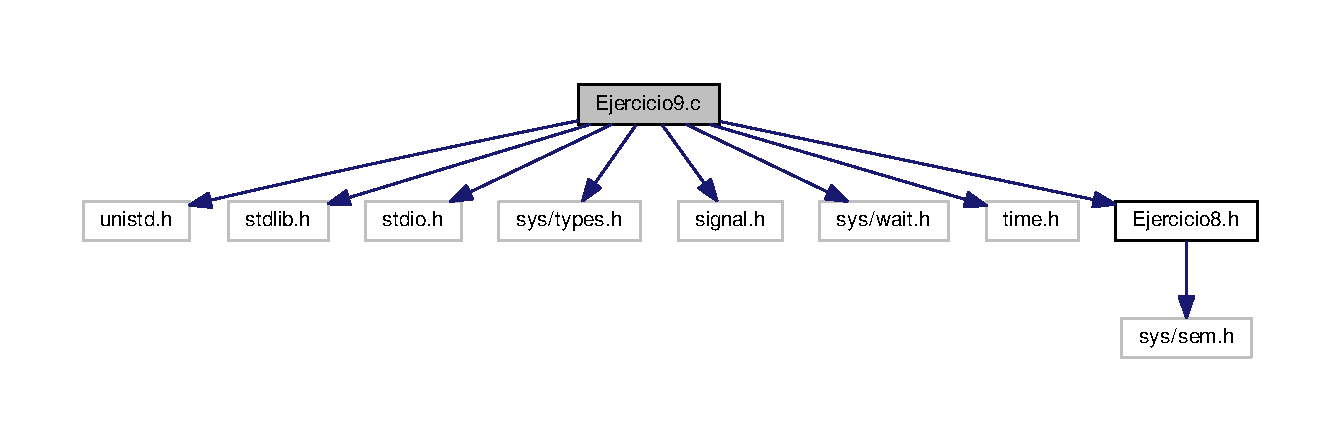
\includegraphics[width=350pt]{Ejercicio9_8c__incl}
\end{center}
\end{figure}
\subsection*{Functions}
\begin{DoxyCompactItemize}
\item 
double \hyperlink{Ejercicio9_8c_a1e86e884e71a85fdafe94dc3ee7f77f8}{potencia} (int a, int b)
\begin{DoxyCompactList}\small\item\em hacemos la operacion matematica a$^\wedge$b \end{DoxyCompactList}\item 
double \hyperlink{Ejercicio9_8c_a5cf432a7c889fe75dffc281247cb867e}{factorial} (int a, int b)
\begin{DoxyCompactList}\small\item\em hacemos la operacion matematica a!/b \end{DoxyCompactList}\item 
double \hyperlink{Ejercicio9_8c_ab13db5a54377e7e55eb6db91185af27e}{num\+Combinatorio} (int a, int b)
\begin{DoxyCompactList}\small\item\em hallamos el numero combinatorio a sobre b de forma recursiva \end{DoxyCompactList}\item 
double \hyperlink{Ejercicio9_8c_a7d7edaebcf72f07f2ca29c75e69460e1}{suma\+Absoluta} (int a, int b)
\begin{DoxyCompactList}\small\item\em hallamos la suma de a y b en valores absolutos \end{DoxyCompactList}\item 
int \hyperlink{Ejercicio9_8c_ae66f6b31b5ad750f1fe042a706a4e3d4}{main} ()
\begin{DoxyCompactList}\small\item\em Hacemos distintas operaciones matemáticas sobre dos numeros en procesos independientes. \end{DoxyCompactList}\end{DoxyCompactItemize}


\subsection{Detailed Description}
Ejercicio 9. Dados dos numeros pasados en la entrada, calculamos el factorial de uno partido del otro, uno elevado al otro, la suma con valores absolutos y el numero combinatorio de uno sobre todo. Cada operacion se realiza en un proceso distinto, que se comunica con el padre mediante pipes. 

\begin{DoxyAuthor}{Author}
\href{mailto:Javier.delgadod@estudiante.uam.es}{\tt Javier.\+delgadod@estudiante.\+uam.\+es} \href{mailto:Javier.lopezcano@estudiante.uam.es}{\tt Javier.\+lopezcano@estudiante.\+uam.\+es} 
\end{DoxyAuthor}


\subsection{Function Documentation}
\index{Ejercicio9.\+c@{Ejercicio9.\+c}!factorial@{factorial}}
\index{factorial@{factorial}!Ejercicio9.\+c@{Ejercicio9.\+c}}
\subsubsection[{\texorpdfstring{factorial(int a, int b)}{factorial(int a, int b)}}]{\setlength{\rightskip}{0pt plus 5cm}double factorial (
\begin{DoxyParamCaption}
\item[{int}]{a, }
\item[{int}]{b}
\end{DoxyParamCaption}
)}\hypertarget{Ejercicio9_8c_a5cf432a7c889fe75dffc281247cb867e}{}\label{Ejercicio9_8c_a5cf432a7c889fe75dffc281247cb867e}


hacemos la operacion matematica a!/b 

\hyperlink{Ejercicio9_8c_a5cf432a7c889fe75dffc281247cb867e}{factorial(int a, int b)} hacemos factorial 
\begin{DoxyParams}{Parameters}
{\em a} & numero sobre el que hacemos el factorial \\
\hline
{\em b} & cociente de la opercion \\
\hline
\end{DoxyParams}
\begin{DoxyReturn}{Returns}
double a!/b 
\end{DoxyReturn}
\index{Ejercicio9.\+c@{Ejercicio9.\+c}!main@{main}}
\index{main@{main}!Ejercicio9.\+c@{Ejercicio9.\+c}}
\subsubsection[{\texorpdfstring{main()}{main()}}]{\setlength{\rightskip}{0pt plus 5cm}int main (
\begin{DoxyParamCaption}
{}
\end{DoxyParamCaption}
)}\hypertarget{Ejercicio9_8c_ae66f6b31b5ad750f1fe042a706a4e3d4}{}\label{Ejercicio9_8c_ae66f6b31b5ad750f1fe042a706a4e3d4}


Hacemos distintas operaciones matemáticas sobre dos numeros en procesos independientes. 

Creamos cuatro procesos y ocho pipes (una de escritura y otra de lectura para cada proceso), de forma que desde el padre enviamos los dos operandos y desde los hijos los resultados para que el padre los imprima.

\begin{DoxyReturn}{Returns}
int que determina si el programa se ha ejecutado o no con exito. 
\end{DoxyReturn}
\index{Ejercicio9.\+c@{Ejercicio9.\+c}!num\+Combinatorio@{num\+Combinatorio}}
\index{num\+Combinatorio@{num\+Combinatorio}!Ejercicio9.\+c@{Ejercicio9.\+c}}
\subsubsection[{\texorpdfstring{num\+Combinatorio(int a, int b)}{numCombinatorio(int a, int b)}}]{\setlength{\rightskip}{0pt plus 5cm}double num\+Combinatorio (
\begin{DoxyParamCaption}
\item[{int}]{a, }
\item[{int}]{b}
\end{DoxyParamCaption}
)}\hypertarget{Ejercicio9_8c_ab13db5a54377e7e55eb6db91185af27e}{}\label{Ejercicio9_8c_ab13db5a54377e7e55eb6db91185af27e}


hallamos el numero combinatorio a sobre b de forma recursiva 

\hyperlink{Ejercicio9_8c_a5cf432a7c889fe75dffc281247cb867e}{factorial(int a, int b)} hacemos el numero combinatorio a sobre b 
\begin{DoxyParams}{Parameters}
{\em a} & numero de elementos del conjunto \\
\hline
{\em b} & numero de elementos a escoger del conjunto \\
\hline
\end{DoxyParams}
\begin{DoxyReturn}{Returns}
double numero combinatorio a sobre b 
\end{DoxyReturn}
\index{Ejercicio9.\+c@{Ejercicio9.\+c}!potencia@{potencia}}
\index{potencia@{potencia}!Ejercicio9.\+c@{Ejercicio9.\+c}}
\subsubsection[{\texorpdfstring{potencia(int a, int b)}{potencia(int a, int b)}}]{\setlength{\rightskip}{0pt plus 5cm}double potencia (
\begin{DoxyParamCaption}
\item[{int}]{a, }
\item[{int}]{b}
\end{DoxyParamCaption}
)}\hypertarget{Ejercicio9_8c_a1e86e884e71a85fdafe94dc3ee7f77f8}{}\label{Ejercicio9_8c_a1e86e884e71a85fdafe94dc3ee7f77f8}


hacemos la operacion matematica a$^\wedge$b 

\hyperlink{Ejercicio9_8c_a1e86e884e71a85fdafe94dc3ee7f77f8}{potencia(int a, int b)} hacemos a$^\wedge$b 
\begin{DoxyParams}{Parameters}
{\em a} & base de la operacion \\
\hline
{\em b} & exponente de la operacion \\
\hline
\end{DoxyParams}
\begin{DoxyReturn}{Returns}
double a$^\wedge$b 
\end{DoxyReturn}
\index{Ejercicio9.\+c@{Ejercicio9.\+c}!suma\+Absoluta@{suma\+Absoluta}}
\index{suma\+Absoluta@{suma\+Absoluta}!Ejercicio9.\+c@{Ejercicio9.\+c}}
\subsubsection[{\texorpdfstring{suma\+Absoluta(int a, int b)}{sumaAbsoluta(int a, int b)}}]{\setlength{\rightskip}{0pt plus 5cm}double suma\+Absoluta (
\begin{DoxyParamCaption}
\item[{int}]{a, }
\item[{int}]{b}
\end{DoxyParamCaption}
)}\hypertarget{Ejercicio9_8c_a7d7edaebcf72f07f2ca29c75e69460e1}{}\label{Ejercicio9_8c_a7d7edaebcf72f07f2ca29c75e69460e1}


hallamos la suma de a y b en valores absolutos 

\hyperlink{Ejercicio9_8c_a5cf432a7c889fe75dffc281247cb867e}{factorial(int a, int b)} hacemos el numero combinatorio a sobre b 
\begin{DoxyParams}{Parameters}
{\em a} & primer operando \\
\hline
{\em b} & segundo operando \\
\hline
\end{DoxyParams}
\begin{DoxyReturn}{Returns}
double valor absoluto de a mas valor absoluto de b 
\end{DoxyReturn}

%--- End generated contents ---

% Index
\backmatter
\newpage
\phantomsection
\clearemptydoublepage
\addcontentsline{toc}{chapter}{Index}
\printindex

\end{document}
